\chapter{Design}

	The first aim, while starting the design part, was to produce a set of interfaces which could support not only this particular game, but a various range of games which could base themselves on the same abstract logic.
	In particular, RTS AR kind of games could be easily derived from the classes produced for this project.
	Proceeding with the code development it became clear that this aim was partially infeasible, for example while trying to generalize various type of games (Turn based, Checkpoint based, etc.) and location management, due to Java code rules and limitations in terms of Inheritance and Polymorphism.
	To overcome them, core interfaces and classes should have been heavily reworked, so the aim had been lowered a bit to keep project-independent interfaces only for the really basic concepts.

	\section{Game Rules}
		
		Most of the rules from \textbf{Discworld - Ankh-Morpork} has been kept while translating them into the application; the most notably difference are the player management and the card system removal.
		
		\subsection{Leaders and Units}
		
			While in the original game there were 2-4 players which controlled inanimate minions, now there are 2-5 (possibly more) teams, composed by 1 leader and 4-6 units each.
			The leader will represent the player of the original game, while units are the minions he would have moved; following this idea, the leader will be a strategist which will guide the units, like a player of an RTS game coordinating his units.
			More specifically, leaders of all the teams will be conduced in a room with a PC per person, from there they will be able to see everything that is going on in the game via a web application: ally units, enemy units, their movements during the game, etc.
			The leader will be able to communicate with his units both with text and audio, coordinating them and reporting the enemy moves.
			They will as well be the managers of the team money reserve, lending coins to units at the start of the turn and collecting them back at the end of it if not used.
			A part of the role management will also depend by leaders, as described below.
		
		\newpage
		
		\subsection{Board and Zones}\label{design:board}
		
			\begin{table}[htp]
				\caption{Power-up description}
				\label{powup:desc}
				\centering
				\begin{tabular}{lccp{0.5\textwidth}}
					\toprule
					Name 			& N° in game& Cost 	& Description \\
					\midrule
					Money 			& 2 		& 4 	& It adds 3 coins to the team reserve \\
					Money 			& 2 		& 7 	& It adds 5 coins to the team reserve \\
					Calm 			& 1 		& 7 	& If the zone with this power-up is chaotic, calm it down. Otherwise, calm a nearby chaotic zone: if more than one is eligible, the zone to calm down is randomly chosen between the available ones \\
					Role 			& 2 		& 4 	& It adds one extra cop, assassin and builder role in the team role pool \\
					Untouchable 	& 1 		& 9 	& It adds an untouchable bonus role to the team role pool: the player who get this cannot be killed \\
					Multitasking 	& 1 		& 9 	& It adds a multitasking bonus role to the team role pool: the player who get this can use both his actions \\
					\bottomrule
				\end{tabular}
			\end{table}
		
			Board concept has been retained unchanged from the original game, but instead of a physical one in cardboard, a virtual one is generated on-the-fly starting from given centre and radius.
			The algorithm currently generates a pseudo-circular board with nine zones displaced in a symmetric way, with a central zone, 4 zones on the inner ring and 4 zones in the outer ring shifted by 45° with respect to the inner one.
			
			\begin{figure}
				\centering
				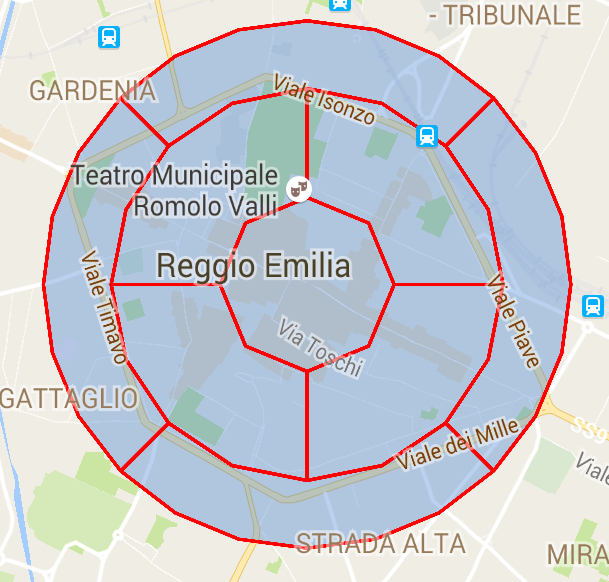
\includegraphics[width=.5\textwidth]{rightboard}
				\caption{Ideal shape of the board and zones}
			\end{figure}
			
			Zones all have the same area, thanks to an R simulation which calculated the right radius to use for different coordinates rings.
			Ideally, moving from a zone centre to another one takes 5 minutes and turn duration is related to this measure: players shall make a choice between moving slightly (one zone or even staying in the same zone) and get plenty of time to perform their actions or move a lot (two or three zones) and risking to run out of time.
			Zones grants a power-up when teams build on each of them (higher the building cost, more useful is the power-up) and they are randomly distributed on the board (e.g., the power-up disposition will be unlikely to be repeated in subsequent games).
			Power-ups activate at the beginning of every turn.
			
			With a board composed by 9 zones, power-ups are defined as described in \autoref{powup:desc}; notice that some of them are referred to the role system explained in the next subsection.
		
		\subsection{Roles and Actions}
		
			The card system had to be removed: while easy to realize and use for single players, it is too complex, time-consuming and random-based to be used in a team-based game, especially if used through an application for mobile devices.
			Removing the card system leaves a hole in the game mechanics related to action assignment. To fill this hole, a new system based on roles was prepared; the main goals of the new system is to leave enough freedom of act to units, removing the feeling of just being minions controlled by the leaders, and create a balanced game play.
			
			In this system only three main roles and a filler one, always available, can be used; all roles have their actions and visibility rule particularities.
			Each role, except the filler one, shall select an action between the two provided.
			The technical implementations of actions are explained in \autoref{focus:augmented:actions}.
		
			\begin{description}
				\item[cops] can see their team mates and all assassins in the zone.
					\begin{description}
						\item[protect] allies units within a certain range can be protected to prevent an assassination.
						\item[calm down] following a path of randomly generated coordinates inside the current zone it won't be chaotic any more.
					\end{description}
				\item[assassins] can see their team mates and all builders in the zone.
					\begin{description}
						\item[assassinate] if the zone is chaotic and he manages to stay within a certain range and a certain time to an enemy, that enemy will become a collector for the rest of the turn, losing his previous action. If the assassinated unit owns coins, the assassin robs them.
						\item[tear down] demolish a building; the owner team get refunded with half the price of the building and lose the zone power-up.
					\end{description}
				\item[builders] can see all other units in the zone, but does not know their role.
					\begin{description}
						\item[build] can be performed only if the zone is not chaotic and the builder carries with him enough money; the builder must stay near a randomly generated point in the current zone for a certain amount of time and playing a small mini-game; if he wins the mini-game, the construction cost is paid and a building rise there, granting a power-up for his team.
						\item[spread panic] following a path of randomly generated coordinates inside the current zone, it will become chaotic.
					\end{description}
				\item[collectors] can see only their team mates and coins positions in the current zone, but he knows the number of the other collectors in it.
					\begin{description}
						\item[collect money] every time he reaches a coin location, he earns one coin. Coins positions are shared between all teams and spawn randomly on the board at the beginning of the turn.
					\end{description}
			\end{description}
			
			Roles had been defined to counter each other: cops can prevent the assassins to do their job, assassins are mainly equipped to attack builders and tear down what they made and builders hinder cops work by spreading the panic in a zone or trying to get its power-up.
			
			Some special roles, called bonus or enhancer roles, are earned as a consequence of particular power-ups and can be assigned by the leader to their units, extra to the one usually distributed.
			Those roles change some in-game rules for their owners:
			\begin{description}
				\item[untouchable] the unit cannot be killed either by assassins or events;
				\item[multitasking] the unit can perform both the actions of the primary role he chose.
			\end{description} 
			
			Role system is managed by leaders and units together.
			At game start units own three roles (one per type) and leaders own six roles (two per type).
			During the start of each turn except the first leaders must give a role to every unit, taken from their role pool, and units will decide which role and associated action will use for that turn.
			At the end of each turn every unit who used its action successfully will refund the spent role, which will be added to the leader role pool, ready to be redistributed on the following phase; if the unit gets assassinated or does not use the action he chose, the role will still be added to the leader pool, but on the subsequent turn.
			
			This system had been thought to give the leaders a way to “set the path” for his units, but still letting them decide independently if they think that a different action could be more useful in that moment.
		
			% INSERT ROLE SYSTEM IMAGE HERE
			
			When giving out roles, leaders can also assign a mission to every unit which consist of a role, an action and a target (another unit or a zone).
			The unit can decide to accept the mission or to ignore it. If the unit decides to accept it, its role and actions are set automatically to the suggested ones and he will see additional informations about its target (his positions, how many units are in the particular area, etc.) depending on the mission nature. If he accomplishes it, the team gain a small money bonus.
			
		\subsection{Starting zones}
			
			Many ideas had been evaluated to decide how the units should start, the main ones were: 
			
			\begin{enumerate}
				\item following the original game, three fixed zones shall be the starting ones for every team, with the units equally distributed on them;
				\item all units start in the central zone;
				\item units start from three fixed zones, but divided by team, instead of being equally distributed.
			\end{enumerate}
			
			The first option is a problem in terms of organization, because every team start already divided and cannot make plans before the game start, thus bounding even more the units to instructions and suggestion given by the leader.
			But on another level, is the option that grants the more equilibrated start in terms of interaction between teams.
			
			The second one seems funny at a first glance, but it can easily result in havoc. Just few units will actually succeed in their action for the first and second turn, slowing down the game.
			
			The third option has the exact opposite effect: for the first turns, teams will not interact at all or do it just a bit, building on the zones near their starting one or collecting money, thus crippling the game at the beginning and giving a feeling of boredom. 
			
			Eventually, the first option was selected for testing, even if the starting zones are now being randomly chosen instead of being fixed.
			% REVIEW, POWER-UP ARE STILL FIXED
			In fact, the main reason for which they were fixed in the first place, was that also the power-ups were fixed: now that the power-up disposition can be randomly generated, the starting zone can be randomly chosen as well.
			
			All starting zones are set as chaotic by default.
		
		\subsection{Objectives}
			
			The objective system, which assigned a different one to every player, has been retained and most of the objectives are inspired to the ones of the board game. Leaders do not know which team has which objective (except its own, obviously), but can deduce it from other teams actions and behaviour, since they will be informed of all objectives in play, and try to hinder other teams.
			
			The objectives are defined as:
			\begin{description}
				\item[chaos] seven zones are chaotic;
				\item[peaceful] there are no chaotic zones or it is the eighth turn and nobody won;
				\item[omnipresent] there is at least one active unit (which has not been killed in the previous turn) or building on at least eight different zones;
				\item[control] the team controls (the sum of the number of its units plus the number of the buildings in a zone is higher of the same sum of every other team) four zones;
				\item[rich] the sum of the team money reserve and the value of all team buildings cost is at least of 50 coins.
			\end{description}
			
			It is important to remind that objective accomplishment is checked at the beginning of each turn: the team must keep the victory condition true until the current turn ends.
			
		\subsection{Random events}
			
			The random events effect did not change much from the original game, but their occurrence, which was bound to the card system, had to be updated. Now the event occurrence is related to a certain probability which increase every turn in which no event takes place, and reset to a minimum when one of them actually does.
			
			The events are defined as:
			\begin{description}
				\item[a drake attack the city] all buildings in a randomly extracted zone are destroyed and all units currently there die;
				\item[a fire breaks out] buildings in a randomly extracted zone are destroyed and another zone is extracted. If this new zone is nearby the previous one and contains buildings, the fire spreads and they are destroyed as well, then keep extracting a new zone until it stop spreading;
				\item[the fog falls on the city] visibility of each player toward others is blocked, both of team mates and enemies, unless they are within a small radius;
				\item[an explosion take place] buildings in in a randomly extracted zone are destroyed;
				\item[time to pay taxes] every team must pay 3 coin for every building it owns or destroy it. Payment is done automatically in zone number order;
				\item[suddenly, earthquake] extract two zones, all building in there are destroyed;
				\item[a political disaster] extract a zone, since now the power-up of that zone is disabled for the entire match;
				\item[demons from below] extract five zones, a demon appears on each of zones, more demons can appear in the same zone. As long as a demon is in it, the zone power-up is disabled, no coins are generated and it is not possible to build. Demons can be killed by assassins via an AR mini-game and have multiple lives.
			\end{description}
			
			Note that when is expressed that buildings are \emph{destroyed}, instead of demolished or tore down, it is meant that the owner team lose the power-up and get no refund; likewise, when is expressed that a unit \emph{dies}, instead of assassinated, it is meant that it loses all the money it was carrying and its role is automatically changed to collector.
			
			
		\subsection{Turns}
		
			The turn mechanics risked being cut off the final version of the game, because it slows down the game with respect to a system much fluid and free.
			It was kept to synchronize phases (e.g., money management, etc.) and avoid problems with the role system: the role refunding would not work in an environment in which all roles did not return to the leader in the same moment to be distributed again.
			
			Every turn is divided in two sub-turns: leaders turn, which last 5 minutes and in which all the team management is concentrated, and units turn, which lasts 15 minutes and in which the real game takes place.
			The basic idea is that leaders will have the 15 minutes of units' turn, while helping them, to define a strategy for next turns; in this way the 5 minutes of their turn are used just to formalize and put in place the strategy previously defined.
			
			This is obviously needed also to prevent units from staying still for too much time; that leads to boredom and ruins the perpetual tension feeling on which the game is based.
			
	\section{Variations}
		
		Playing the game described above requires a high team coordination; some variations had been prepared to simplify the game and address some mechanics which can be too hard to get for new players.
		In particular, the fact that leaders do not physically act in the game is a problem for various reasons:
		
		\begin{itemize}
			\item a good preparation and knowledge of the game rules is needed to be able to lead the team to victory; it is hard to achieve this task in events like the one imagined, because leaders have only few hours to prepare and study the rules: definitely not enough;
			\item staying in a closed room being the mastermind of your group can be stimulating for someone, but there is a possibility that leaders will instead feel isolated and not actively participating to the game;
			\item leader participation requires a web application development and deployment to test also the units part, but this thesis is about the mobile application and the game in itself: adding it would only slow down the production;
			\item an application entirely running on smart phone does not require providing any hardware, while using a web application 4-5 computer are needed.
		\end{itemize}
		
		\newpage
		
		\subsection{Limited leaders}
		
			One possible way to address those problems is to reduce leader's duties distributing the team management to every unit: this removes the web application need.
			In this scenario, leaders plays with their team as they were mere units choosing a role and an action, lose the vision of everything (they only see their team units position) and in general they now look more alike to an on-the-field sergeant or a super-unit than a high level strategist.
			They keep managing the team money reserve and role assignment, but from now on the role pool will be smaller and the system simpler, there won't be missions, for example.
			
			This resolves most of the issues: leaders are now playing with others team members and are more involved in the game; no web application is needed (and thus no computers) and they do not need an in-depth knowledge of the game rules, because they are required only to manage money and a simplified role system.
		
		\subsection{No leaders}
		
			The natural evolution is to remove the leader figure at all.
			Here, teams are formed by peer units which together take on what before were leader duties, helped by the application to do so.
			When the team cannot reach a shared decision, the system will follow a default path or choose randomly between the options, usually resulting a disadvantage to some units or to the entire team: this shall convince the team to collaborate positively.
			
			\textbf{The project will implement this variation of the game.}
			
			% FIXED ROLE POOL?
			\subsubsection{Roles}
			\label{nolead:role}
				Role distribution in this scenario change drastically: role pool is fixed (two roles per type, infinite for the filler role) and the role choice is bounded to a timer.
				Every unit must select its preferred role for that turn, if there are left of that kind, and communicate with the team to resolve possible conflicts (e.g., three units want to be assassins).
				When the timer stops, every unit gets the role he selected, or the collector role if no one had been selected at all, and must choose the action. Conflicts are avoided in a first-come, first-served fashion.
				
				Bonus roles are managed more or less in the same way: players can ask to use one of them \emph{in addition} to their preferred role, and conflicts are avoided in the same way as the normal roles.
							
			\subsubsection{Money}
			\label{nolead:money}
				Money distribution is managed similarly; when the turn starts, units ask to borrow a certain amount of money from the team reserve: if there is enough money for everyone the money is simply distributed to who asked for it, while if the requested money exceeds the team reserve units must discuss to resolve possible conflicts.
				When the turn ends, money from all units is put back into the team reserve.
				
				This could be achieved also by a request on-the-fly only when the money is needed, but this alternative would bring even more problems: the rule that allows assassins to rob their victims partially breaks apart, because only the collectors (or another assassin which had previously killed a collector) will have money with them; additionally loans would probably need a confirmation vote from all others units, wasting a lot of time.
		